% This is samplepaper.tex, a sample chapter demonstrating the
% LLNCS macro package for Springer Computer Science proceedings;
% Version 2.20 of 2017/10/04
%
\documentclass[runningheads]{llncs}
%
\usepackage{graphicx}

\usepackage{amsmath}
\usepackage{amssymb}
\usepackage{hyperref} 
\usepackage{soul}  
\usepackage{color}
\usepackage{xcolor}
\usepackage{graphicx}
\usepackage{inputenc} 
\usepackage{comment}
%\usepackage{wrapfig} 
\usepackage{ae}  
\usepackage{sidecap}
\usepackage{url}
\usepackage[T1]{fontenc} 
\usepackage{verbatim}
\usepackage{listings} 
\usepackage{tikz}
\usepackage{etoolbox}
\usepackage{mdframed}
\usepackage{tabularx}
\usepackage{multirow}
\usepackage{setspace}

\newenvironment{code}
    {\noindent
     \rule{\columnwidth}{0.6pt}
     \vspace{-4mm}
     \scriptsize \verbatim}
    {\endverbatim \normalsize
     \vspace{-4mm} 
    \rule{\columnwidth}{0.6pt} 
 	}
\usepackage{wrapfig}
\usepackage{relsize}
\usepackage{microtype}
\usepackage{multirow}
\usepackage{semantic}

\usepackage{booktabs}
\usepackage{paralist}
% important for nicer code font
\usepackage[scaled]{beramono}

\definecolor{lightlightgray}{gray}{0.9}
\definecolor{codecolor}{gray}{0.15} 
\definecolor{javadocblue}{rgb}{0,0,0.8} % javadoc
\definecolor{blackblack}{rgb}{0,0,0}
  
\definecolor{myGray1}{rgb}{0.85,0.85,.85}

\lstset{
basicstyle=\ttfamily\scriptsize\color{codecolor}, 
keywordstyle=\color{blackblack}\bfseries,       
% keywordstyle=\color{javadocblue},     
commentstyle=\color{gray},              
numbers=none,                           
numberstyle=\tiny,                      % Line-numbers fonts
stepnumber=1,                           % Step between two line-numbers
numbersep=5pt,                          % How far are line-numbers from code
%backgroundcolor=\color{lightlightgray}, % Choose background color
tabsize=2,     
frame=single,
%xleftmargin=1.5mm,
%xrightmargin=1.5mm,
captionpos=b,   
keepspaces=true,
xleftmargin=1.5mm,
xrightmargin=1.5mm,                        % Caption-position = bottom
breaklines=true,    
escapeinside={@}{@},
                    % Automatic line breaking?
breakatwhitespace=false,                % Automatic breaks only at whitespace?
showspaces=false,                       % Dont make spaces visible
showtabs=false,                         % Dont make tabls visible
columns=flexible,                       % Column format
morekeywords={}
mathescape=false
} 


% Used for displaying a sample figure. If possible, figure files should
% be included in EPS format.
%
% If you use the hyperref package, please uncomment the following line
% to display URLs in blue roman font according to Springer's eBook style:
% \renewcommand\UrlFont{\color{blue}\rmfamily}

%\newcommand\parhead[1]{\vspace{1mm}\noindent\textbf{{#1}}\ \ }  
%\newcommand\parheadX[1]{\vspace{-1.0mm}\noindent\textbf{{#1}}\ \ }  

\newcommand{\toolurl}[1]{\footnote{\smaller\url{{#1}}\normalsize}}
\newcommand{\ic}[1]{\changefont{cmtt}{m}{n}{#1}\normalfont}  % inline code
\newcommand{\changefont}[3]{\fontfamily{#1}\fontseries{#2}\fontshape{#3}\selectfont}
\newcommand{\fig}[1]{Fig. \ref{#1}}  % inline code
\newcommand{\sect}[1]{Sec. \ref{#1}}  % inline code

\newcommand\parheadX[1]{\noindent \colorbox{myGray1}{\textcolor{black}{\textsf{\textbf{\footnotesize {#1}}}}}}  
\newcommand\parhead[1]{\vspace{3mm}\noindent \colorbox{myGray1}{\textcolor{black}{\textsf{\textbf{\footnotesize {#1}}}}}}  

\newcommand\todo[1]{\vspace{1mm}\noindent\textbf{\color{red} {{TODO: {#1}} }}}  


\newmdenv[innerlinewidth=1pt, linecolor=black, innerleftmargin=3pt,
innerrightmargin=3pt,innertopmargin=3pt,innerbottommargin=3pt,backgroundcolor=lightlightgray]{mybox}

\newif\ifFullVersion
\FullVersionfalse

\begin{document}
%
\title{Programming \\ vs. \\ That Thing Subject Matter Experts Do}

\titlerunning{Programming vs. SME'ing}

%  \titlerunning{Abbreviated paper title} If the paper title is too long for the
% running head, you can set an abbreviated paper title here
\author{Markus Voelter}
\authorrunning{M. Voelter}
% First names are abbreviated in the running head.
% If there are more than two authors, 'et al.' is used.
\institute{independent/itemis, Oetztaler Strasse 38, 70327 Stuttgart, Germany\\
\email{voelter@acm.org}}
\maketitle              % typeset the header of the contribution
\begin{abstract}
\keywords{Domain Specific Language  \and End-user Programming \and Language Engineering.}
\end{abstract}
%
%
%

% \begin{mdframed}
% \textbf{A note for the ISOLA reviewers.} In my experience, one of the biggest challenges
% of the DSL community is that we have a very hard time convincing people who
% might benefit from using DSLs to actually use one.
% We have all written lots of scientific papers and case studies that demonstrate
% clearly that DSLs are useful, but still we have a hard time breaking through. With
% this paper I'm trying a different approach. It is based on anecdotes, it is hopefully
% easy to read, and it doesn't contain any technical details or data.
% I know that this is not a very
% scientific approach. But I would ask you to read the paper and provide feedback
% relative to the goal: to try and convince programmers to give DSLs a try.
% Because---again---I think this is really what our community needs to move forward.
% \end{mdframed}

\newcommand{\datev}{DATEV}
\newcommand{\voluntis}{Voluntis}
\newcommand{\ohb}{OHB}

\newcommand{\caseend}{$\blacksquare$}

 


\section{The role of subject matter experts}

Subject matter experts, or SMEs, own the knowledge and expertise that is the
backbone of software and the foundation of digitalization. But too often this
rich expertise is not captured in a structured way and gets lost when
translating it for software developers for implementation. With the rate of
change increasing, time-to-market shortening and product variability blooming,
this indirect approach of putting knowledge into software is increasingly
untenable. It causes delays, quality problems and frustration for everybody
involved. A better approach is to empower \emph{subject matter experts} to
capture, understand, reason about data, structures, rules, behaviors and other
forms of knowledge and expertise in a precise and unambiguous form by providing
them with tailored software languages and tools that allow them to directly
edit, validate, simulate and test that knowledge. The models created this way
are then automatically transformed into program code. The \emph{software
engineers} focus their activities on building these languages, tools and
transformations, plus robust execution platforms for the generated code.

\todo{Refer to Manifesto}

\section{(Where) Does this work?}

\todo{Refer to Existing publications on DSL stuff to show this works}

\todo{Discuss my domain-suitability thing}


\section{Can SMEs do that?}

Do SMEs become programmers?
 

\section{Difference between programming and SME'ing}


\begin{figure}
\begin{center}
    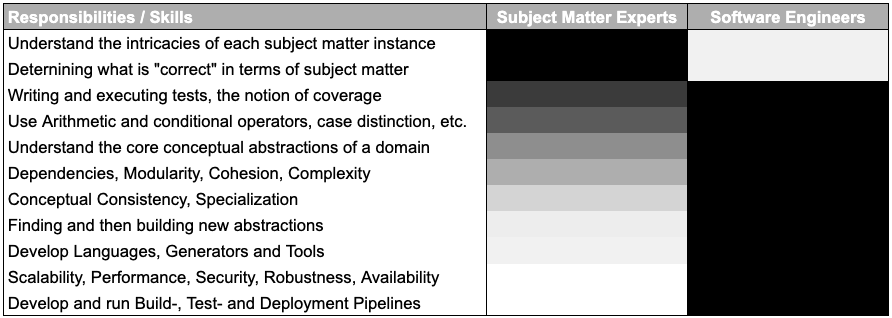
\includegraphics[width=1\columnwidth]{figures/table-respo.png}
    \caption{}
    \label{table-respo}
\end{center} 
\end{figure} 


\section{Where and how to learn}

Comp think
Felienne
Mein Prog Basics stuff






%\section*{Acknowledgements}




\bibliographystyle{abbrv}
\bibliography{doc}

\end{document}